\chapter{Background Theory}

\label{ch:background}

\section{Introduction}

We will cover how deep symbolic reinforcement learning extracts symbolic representations from raw input data, which will motivate a discussion of loss functions and the introduction of autoencoders. Seeing the limitations of the current approach in extracting symbolic representations, we can appreciate the recent development of $\beta$-VAE, a variant of the variational autoencoder used to learn disentangled representations. Finally, we can conclude by mentioning less technical matters, such as libraries and hardware used.

\section{Loss functions}

The idea of image reconstruction plays a vital role throughout this project. Although it's possible to qualitatively compare the original to its reconstruction, it's important to be able to quantify the difference, which lends itself to automation. The loss function will quantify how similar two images are.

To compare loss functions, we'll use the MNIST data set. MNIST is a collection of $70,000$ black-and-white images of handwritten digits. These images will be represented as vectors without loss of generality.

\subsection{Euclidean Distance}

The Euclidean distance between two vectors $\vec{x}$ and $\vec{y}$ is defined by $$\sqrt{\sum_{i}(x_i - y_i)^2}$$ where $x_i$ and $y_i$ are the $i^{th}$ components of $\vec{x}$ and $\vec{y}$ respectively.

\subsection{Mean Squared Error}

The mean squared error of the vector $\vec{x}$ and its target $\vec{y}$, both of length $N$, is defined by $$\frac{1}{N}\sum_{i}(x_i - y_i)^2$$ where $x_i$ and $y_i$ are the $i^{th}$ components of $\vec{x}$ and $\vec{y}$ respectively.

\subsection{Binary Cross-Entropy}
Consider a single black-and-white pixel with probability $p(0) = y$ of being $0$ and $p(1) = 1 - y$ of being $1$. Here $p$ is a probability distribution over the possible pixel values $0$ and $1$. Suppose a given model tries to learn the distribution described by $p$, and says that the pixel has probability $q(0) = \hat{y}$ of being $0$ and $q(1) = 1 - \hat{y}$ of being $1$. The model is perfect if it learns the true distribution, that is, if $q(x) = p(x)$ for $x\in\{0,1\}$. We'd like to quantify how similar the distributions $p$ and $q$ are.

This is done by computing the binary cross-entropy between $p$ and $q$, which is defined by $$H(p,q) = -y\log\hat{y} - (1-y)\log(1-\hat{y})$$

To see how we may use this as a similarity measure among images, consider a $1\times1$ image. Normalising this image yields a pixel value in the interval $[0, 1]$, which may now be interpreted as a probability, corresponding to $y$ above. In the normalised reconstructed image, the pixel value corresponds to $\hat{y}$. We simply compute the binary cross-entropy to measure the similarity of these two distributions, and in turn, the similarity of the images themselves! (Note: we could have also assigned the probabilities to $1-y$ and $1-\hat{y}$ by symmetry of binary cross-entropy).


\section{Autoencoders}

An autoencoder is a neural network that learns a compression algorithm for its input data in an unsupervised manner \cite{Liou2008}. This is achieved by placing constraints on a hidden layer, called the latent space, and setting the target values to the input, effectively learning the identity function. Since the network is trying to reconstruct the original input from the constrained latent space, over time the latent space corresponds to a meaningful compression of the network's input.

There are a number of architectures implementing the same concept

\subsection{Fully-Connected Autoencoders}

\begin{figure}[h!]
\centering
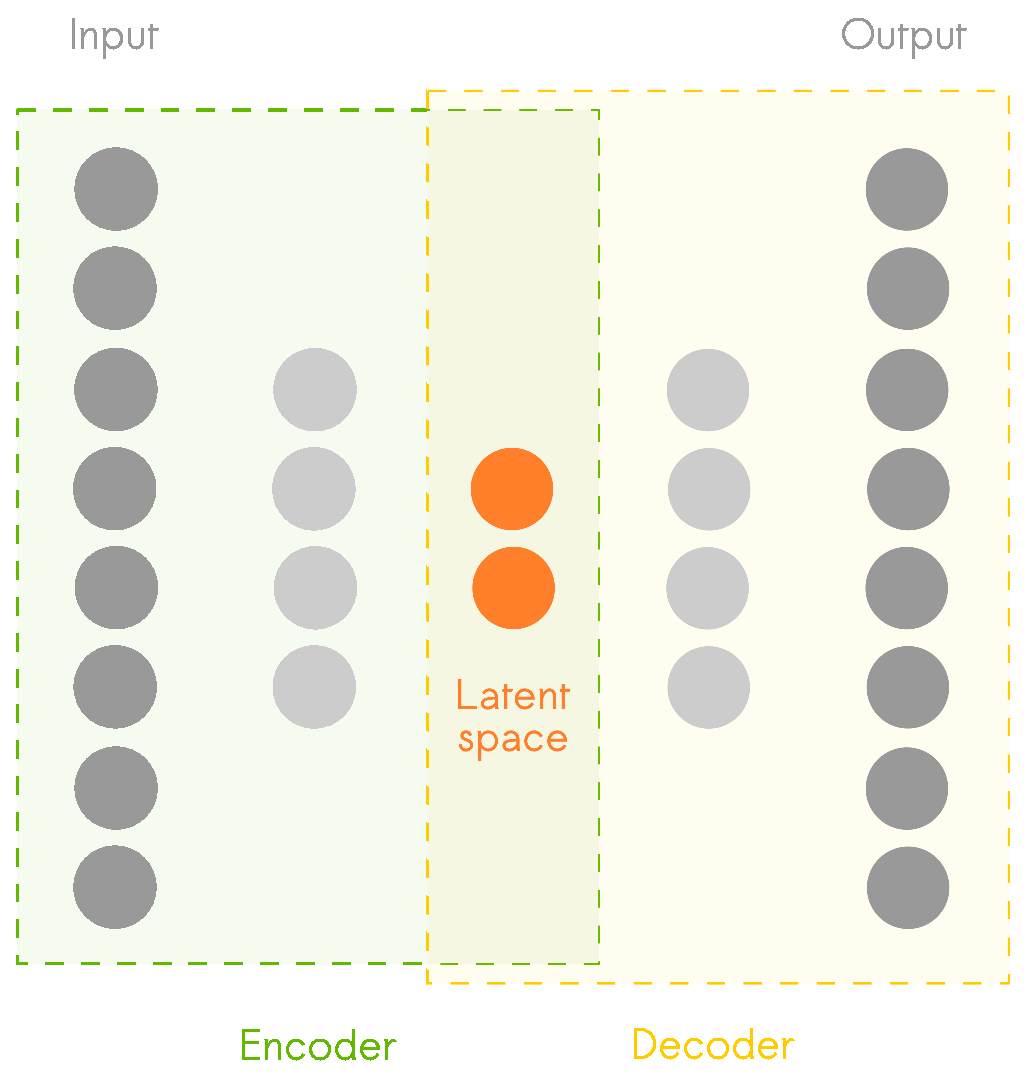
\includegraphics[scale=0.7]{background/autoencoder_architecture.eps}
\caption{Architecture of an autoencoder.}
\end{figure}

\subsection{Convolutional Autoencoders}

\subsection{Variational Autoencoders}